\documentclass{article}
\usepackage[utf8]{inputenc}
\usepackage{subfig}
\usepackage{amsmath}
\usepackage[export]{adjustbox}
\usepackage{graphicx}
\usepackage[legalpaper, landscape, margin=0.5cm]{geometry}

\thispagestyle{empty}
% \renewcommand{\thesubfigure}{\roman{subfigure}}
\begin{document}

\begin{figure}[h]
        \centering
        \subfloat[-40 mm]{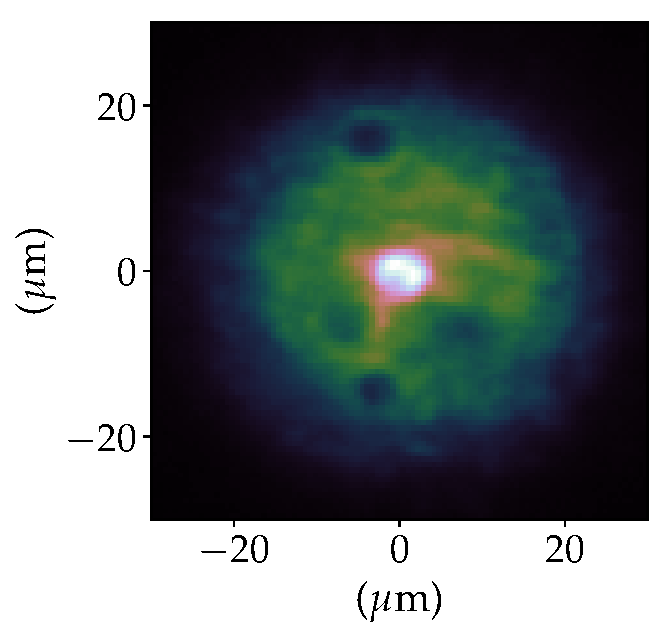
\includegraphics[height=3.cm]{figures/ch06/experimental/a2scan_Mo_again2_0032.pdf}}
        \subfloat[-30 mm]{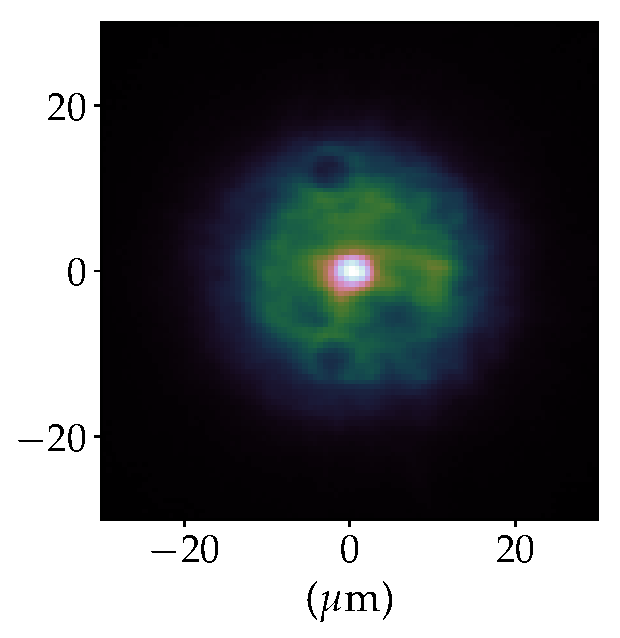
\includegraphics[height=3.cm]{figures/ch06/experimental/a2scan_Mo_again2_0037.pdf}}
        \subfloat[-20 mm]{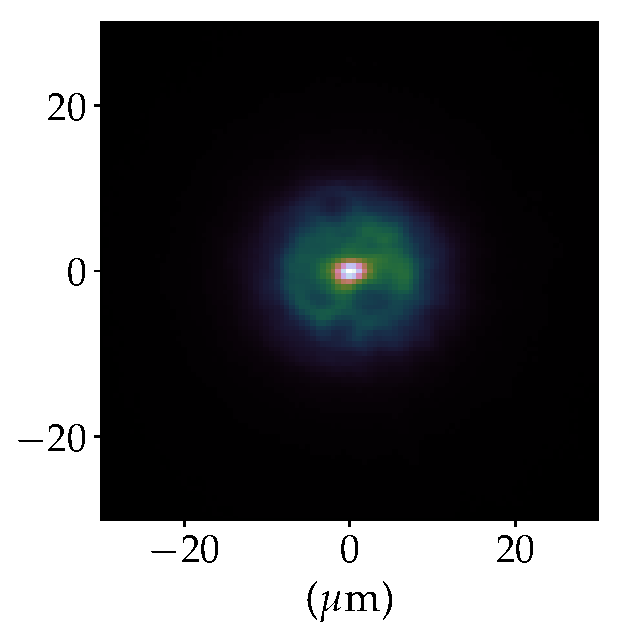
\includegraphics[height=3.cm]{figures/ch06/experimental/a2scan_Mo_again2_0042.pdf}}
        \subfloat[-10 mm]{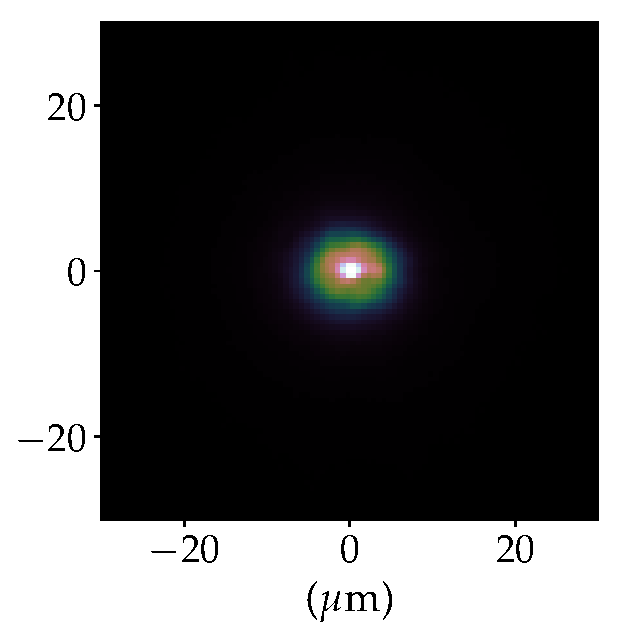
\includegraphics[height=3.cm]{figures/ch06/experimental/a2scan_Mo_again2_0047.pdf}}
        \subfloat[+10 mm]{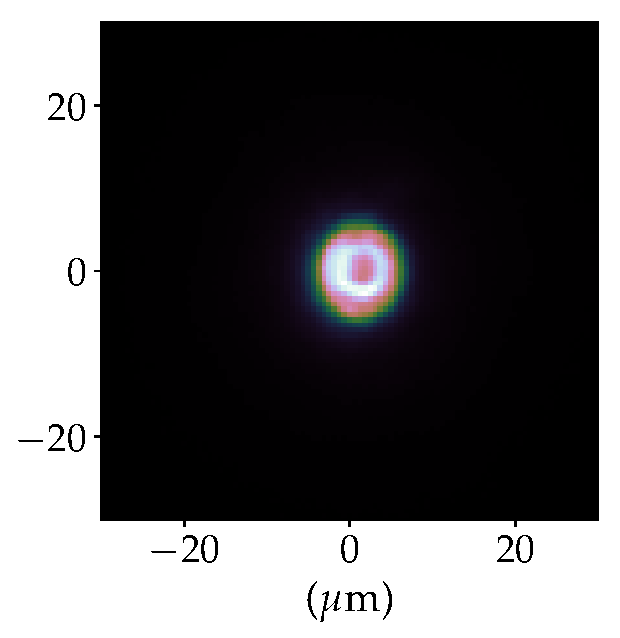
\includegraphics[height=3.cm]{figures/ch06/experimental/a2scan_Mo_again2_0057.pdf}}
        \subfloat[+20 mm]{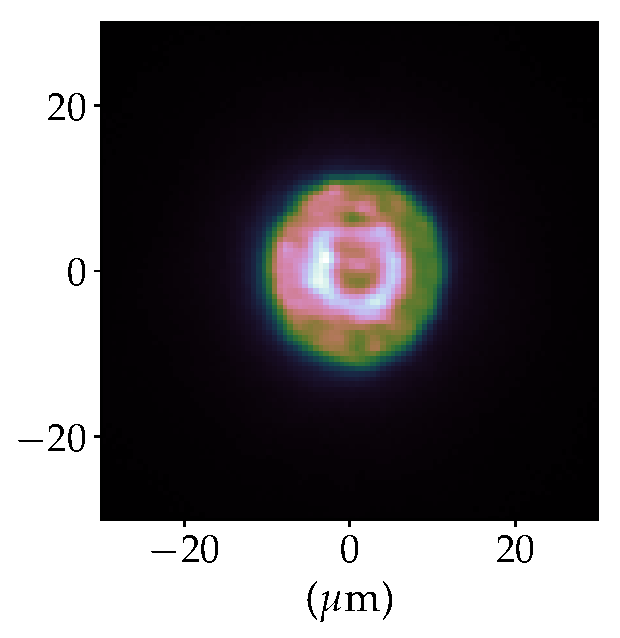
\includegraphics[height=3.cm]{figures/ch06/experimental/a2scan_Mo_again2_0062.pdf}}
        \subfloat[+30 mm]{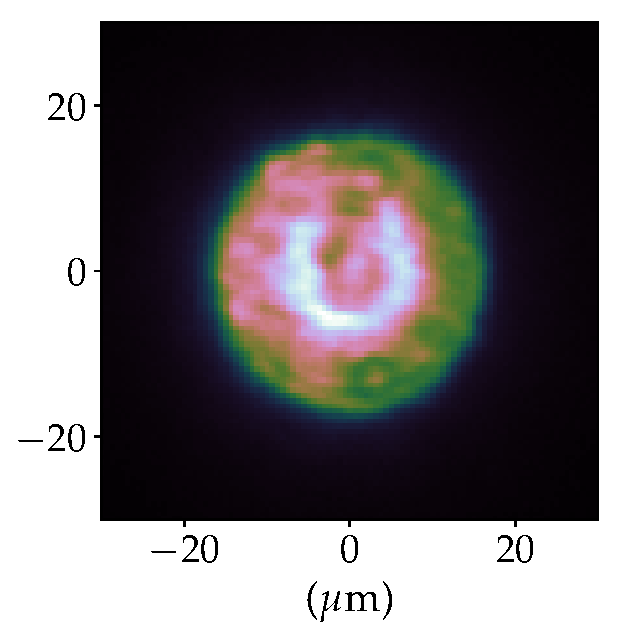
\includegraphics[height=3.cm]{figures/ch06/experimental/a2scan_Mo_again2_0067.pdf}}
        \subfloat[+40 mm]{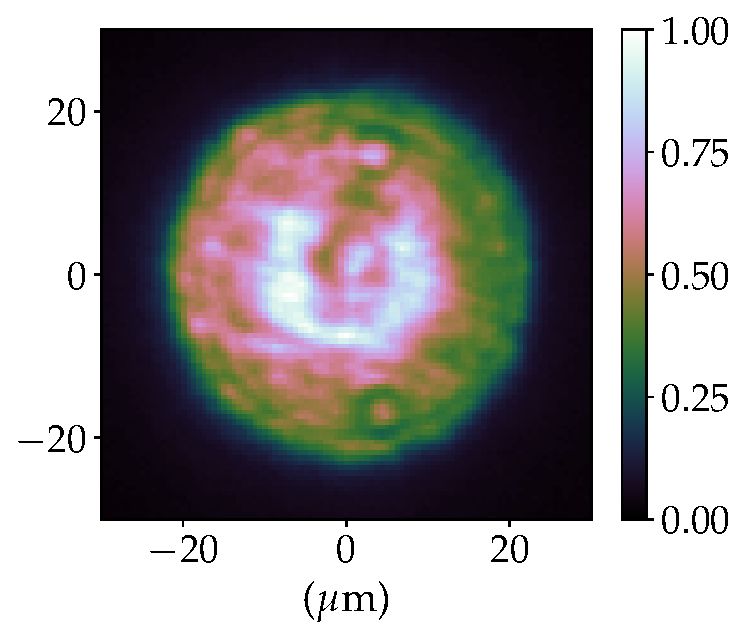
\includegraphics[height=3.cm]{figures/ch06/experimental/a2scan_Mo_again2_0072.pdf}}\\
        \subfloat[beam caustics]{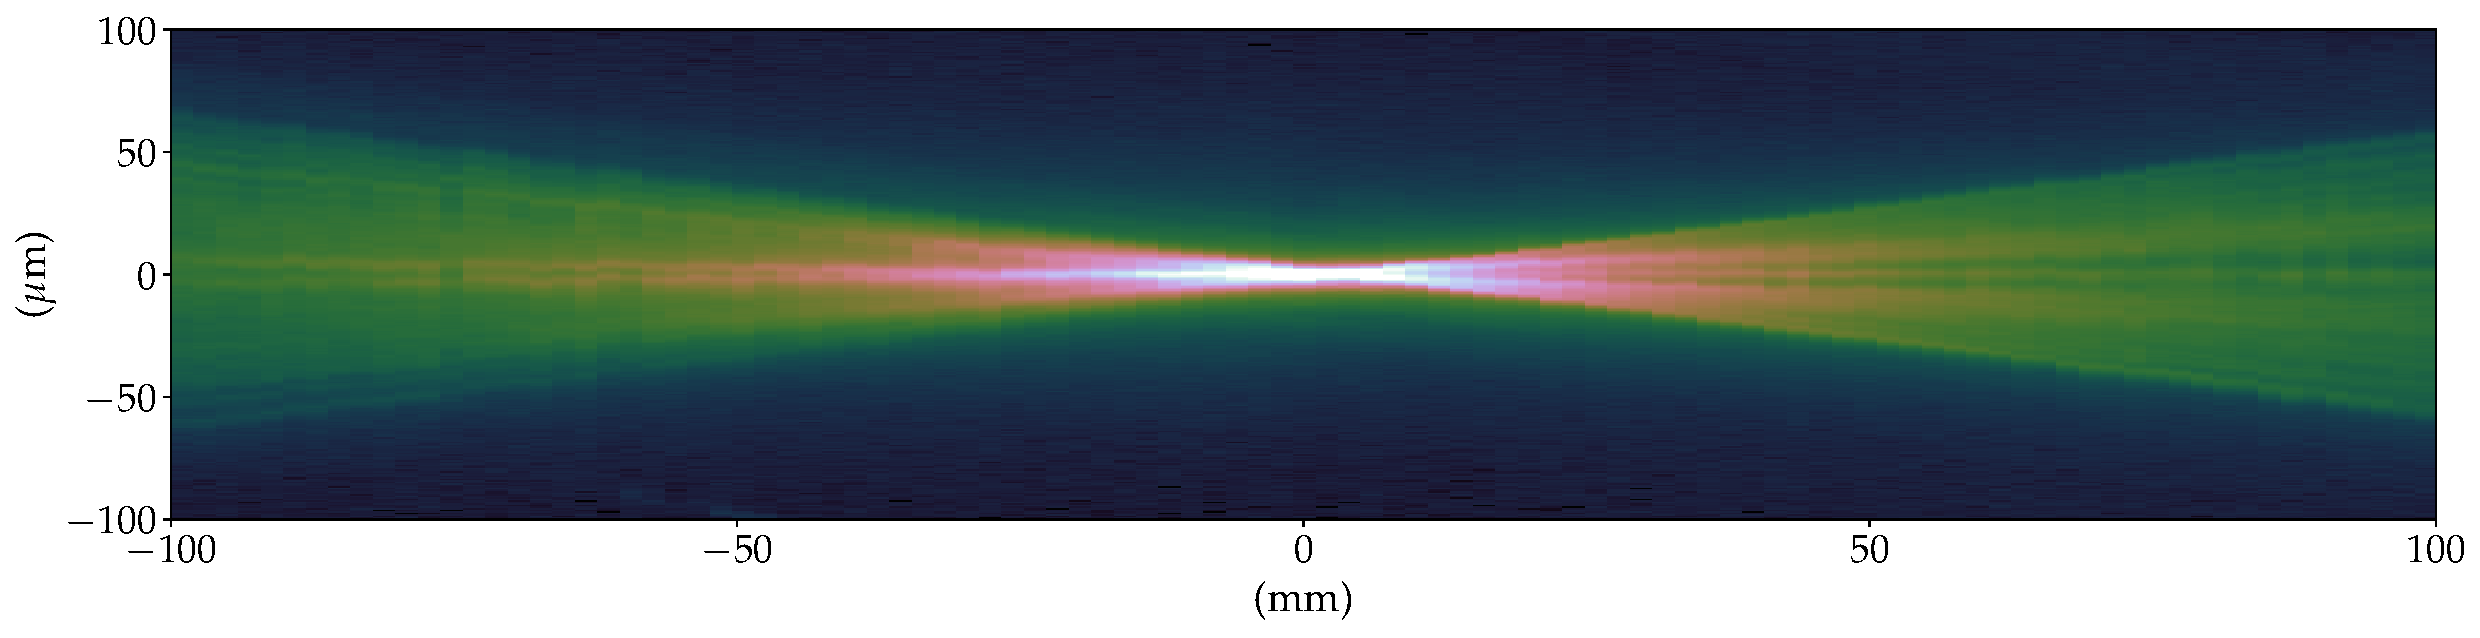
\includegraphics[height=3.5cm]{figures/ch06/experimental/CDn_cst_cut_x_a2scan_Mo_again2_full.pdf}}\hspace{0.1cm}
        \subfloat[zoomed beam caustics]{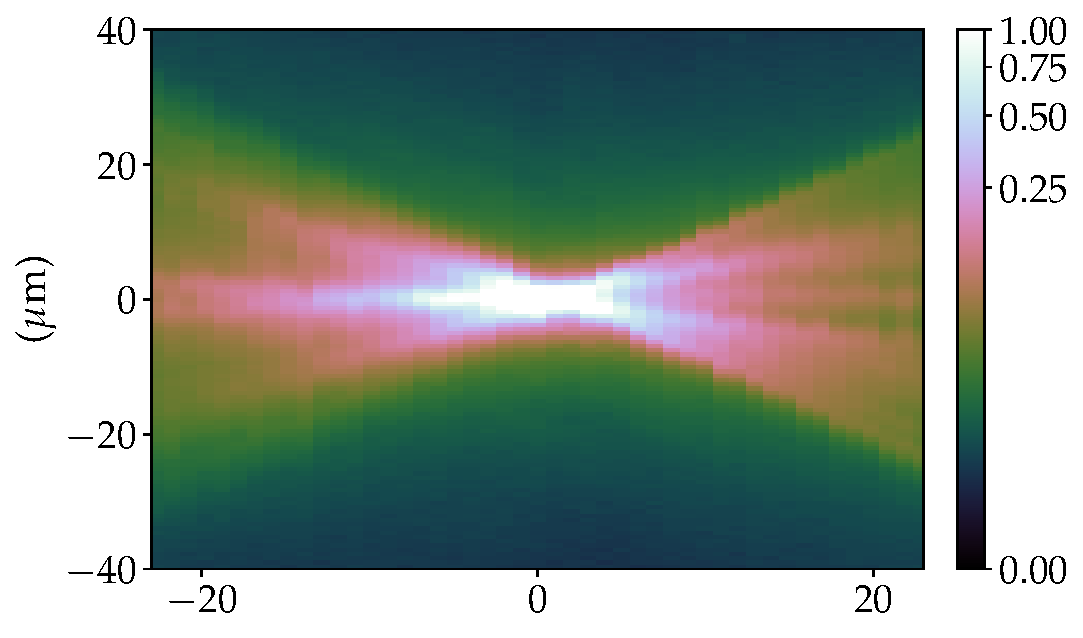
\includegraphics[height=3.5cm]{figures/ch06/experimental/CDn_cst_cut_x_a2scan_Mo_again2_reduced.pdf}}\\
        \caption*{aberrated system}\setcounter{subfigure}{0}
        \subfloat[-40 mm]{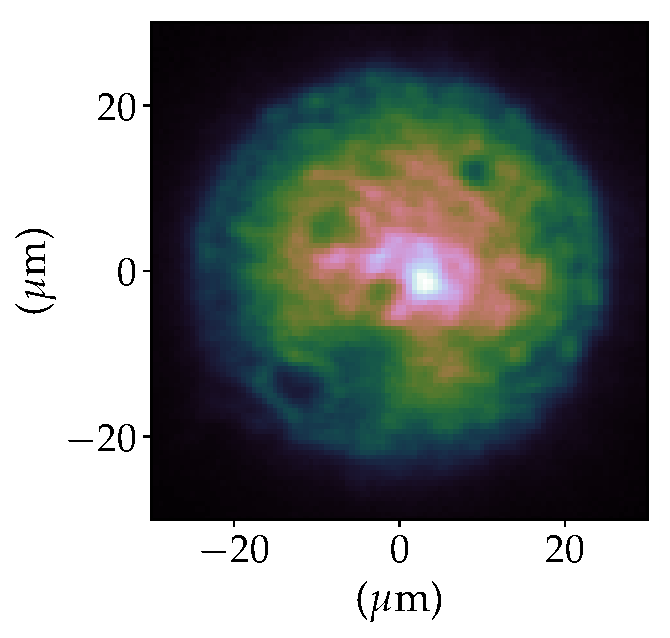
\includegraphics[height=3.cm]{figures/ch06/experimental/N10R50p5_outOfFocus_a2scan_Mo0306.pdf}}
        \subfloat[-30 mm]{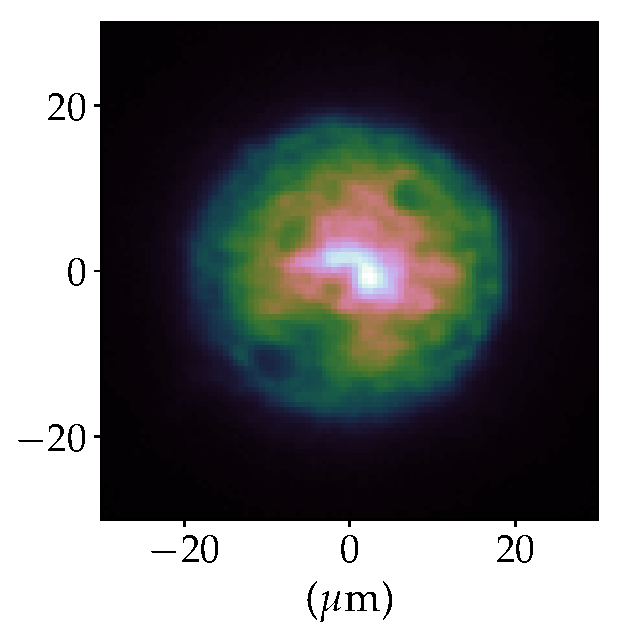
\includegraphics[height=3.cm]{figures/ch06/experimental/N10R50p5_outOfFocus_a2scan_Mo0301.pdf}}
        \subfloat[-20 mm]{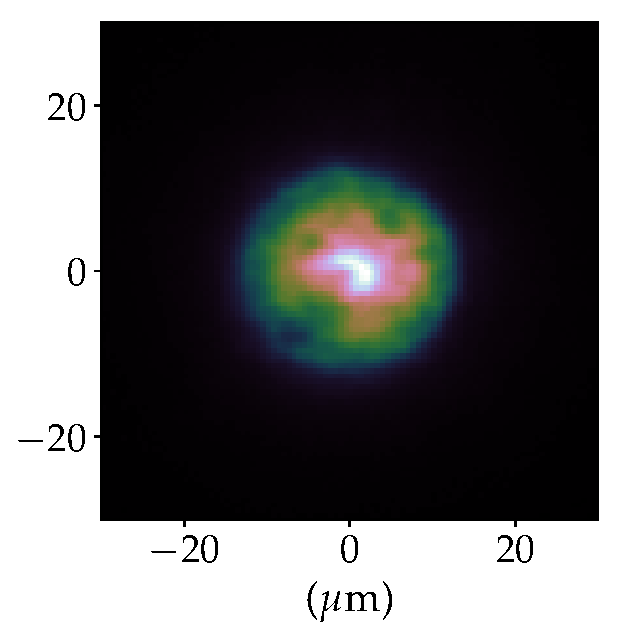
\includegraphics[height=3.cm]{figures/ch06/experimental/N10R50p5_outOfFocus_a2scan_Mo0296.pdf}}
        \subfloat[-10 mm]{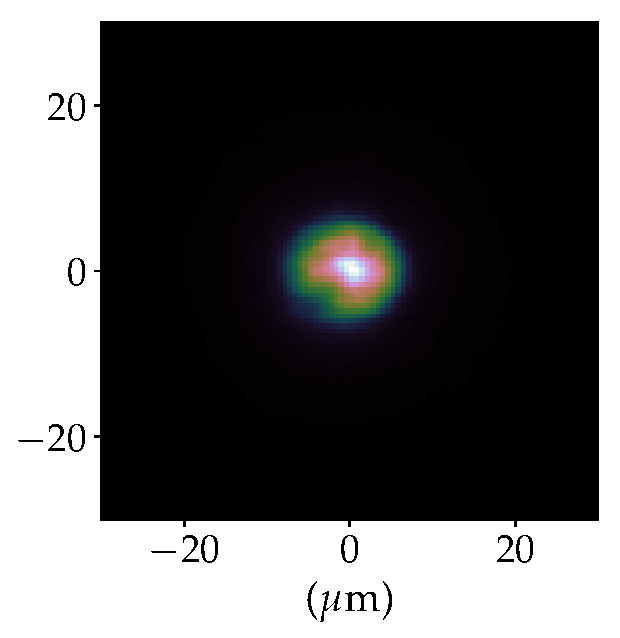
\includegraphics[height=3.cm]{figures/ch06/experimental/N10R50p5_outOfFocus_a2scan_Mo0291.pdf}}
        \subfloat[+10 mm]{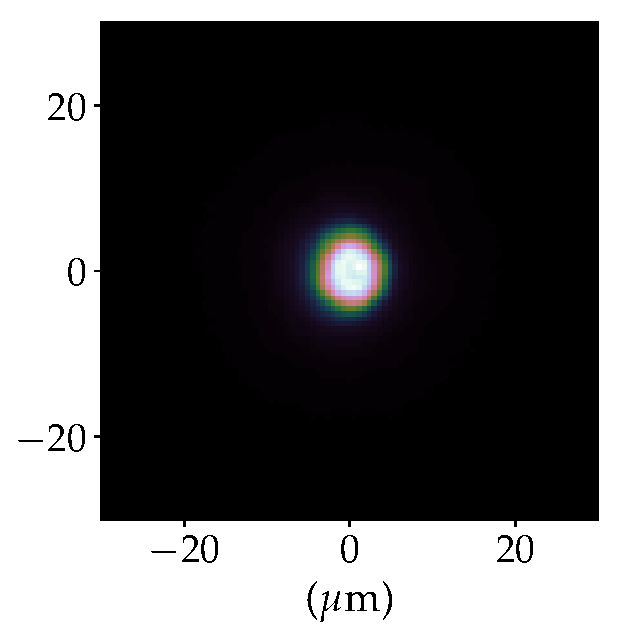
\includegraphics[height=3.cm]{figures/ch06/experimental/N10R50p5_outOfFocus_a2scan_Mo0281.pdf}}
        \subfloat[+20 mm]{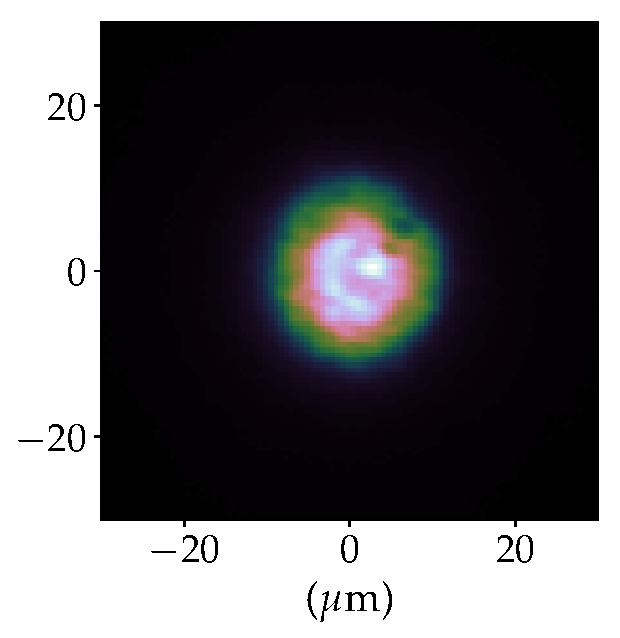
\includegraphics[height=3.cm]{figures/ch06/experimental/N10R50p5_outOfFocus_a2scan_Mo0276.pdf}}
        \subfloat[+30 mm]{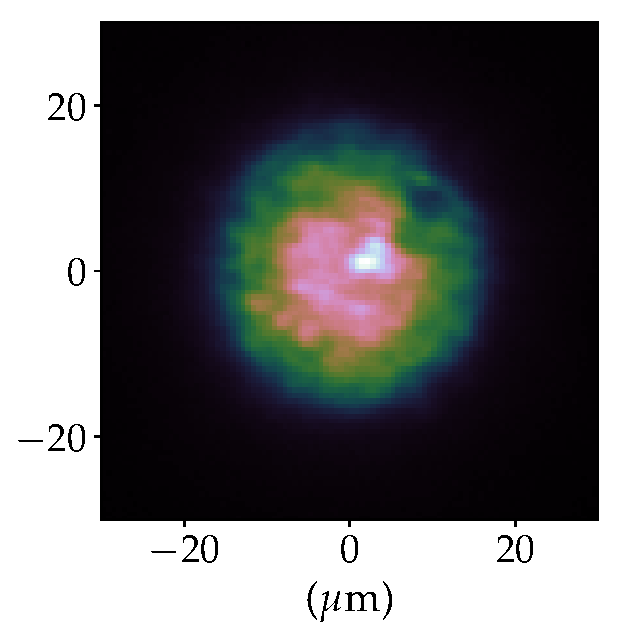
\includegraphics[height=3.cm]{figures/ch06/experimental/N10R50p5_outOfFocus_a2scan_Mo0271.pdf}}
        \subfloat[+40 mm]{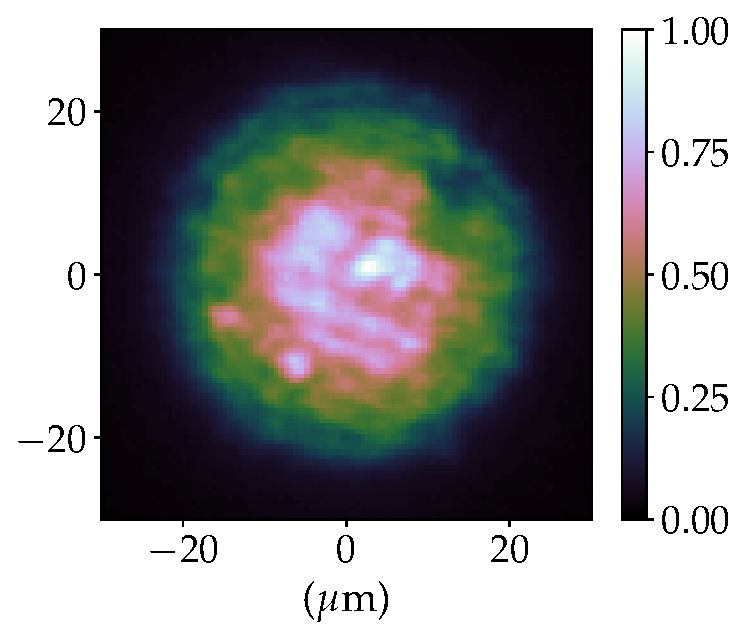
\includegraphics[height=3.cm]{figures/ch06/experimental/N10R50p5_outOfFocus_a2scan_Mo0266.pdf}}\\
        \subfloat[beam caustics]{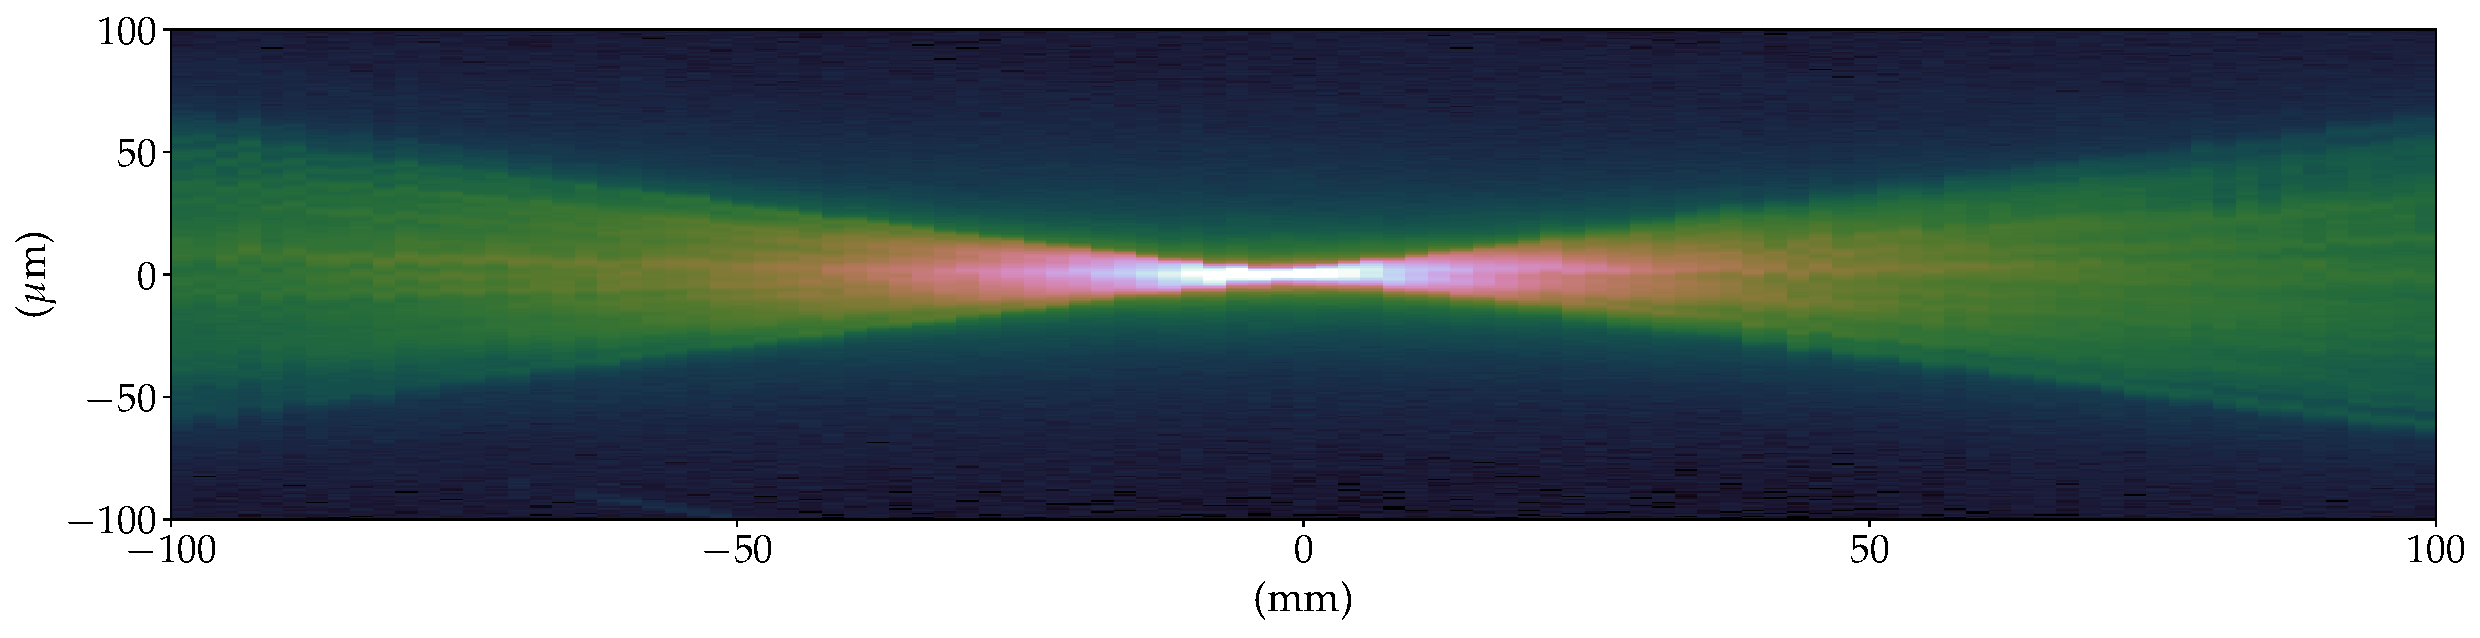
\includegraphics[height=3.5cm]{figures/ch06/experimental/CDn_cst_cut_x_N10R50p5_outOfFocus_a2scan_Mo_full.pdf}}\hspace{0.1cm}
        \subfloat[zoomed beam caustics]{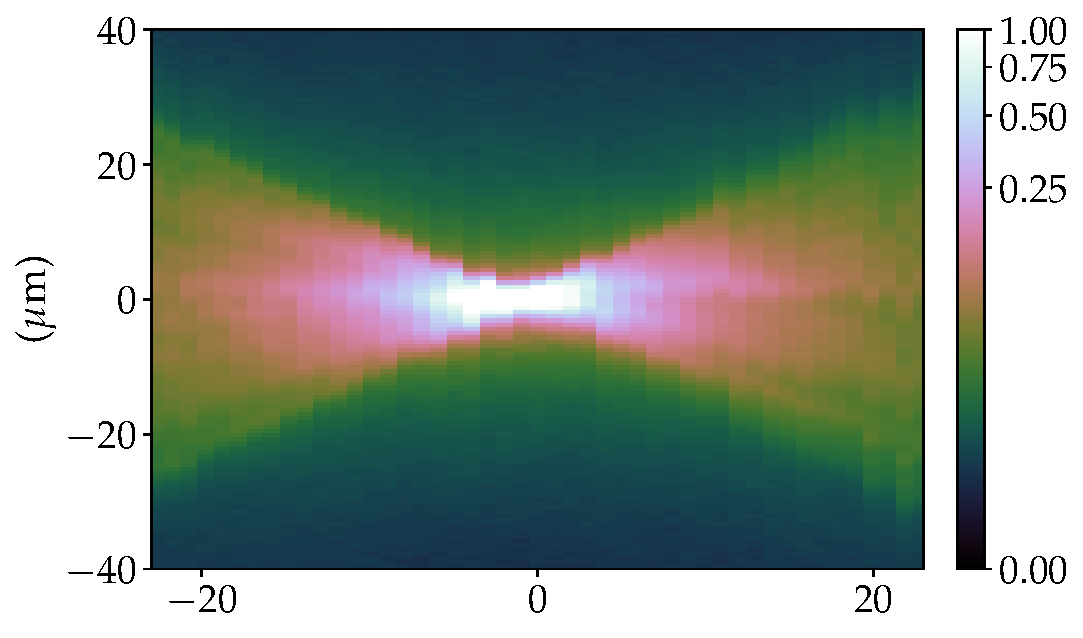
\includegraphics[height=3.5cm]{figures/ch06/experimental/CDn_cst_cut_x_N10R50p5_outOfFocus_a2scan_Mo_reduced.pdf}}
        \caption*{corrected system}\setcounter{subfigure}{0}

\end{figure}
\end{document}